\documentclass{article}
\usepackage[latin1]{inputenc}
\usepackage{amsmath}
\usepackage{amssymb}
\usepackage[algo2e]{algorithm2e}
\usepackage{pgf}
\usepackage{tikz}
\usepackage{verbatim}
\usetikzlibrary{arrows,automata}

\begin{document}

\title{Tools and Algorithms for Deciding Timed Relations}

\author{Mihir Mehta\\
  Department of Computer Science and Engineering,\\
  Indian Institute of Technology, Delhi.\\
  \texttt{cs1090197@cse.iitd.ac.in}
}

\date{April 2013}

\maketitle

\begin{abstract}
  This is a report summarising the author's project on their B Tech
  Project for the academic year 2012-2013.
\end{abstract}

\section{Objectives}

The work described in this thesis builds on the work of
\cite{DBLP:conf/cav/GuhaNA12} in which Guha et al described an
algorithm to generate \emph{zone-valuation graphs} for timed automata
and an algorithm to use such zone-valuation graphs to perform an
on-the-fly analysis to determine \emph{timed performance
  prebisimilarity} on pairs of timed automata. Our aim was to
implement these algorithms in a generalised manner in order to verify
various other timed relations, such as time abstracted bisimulations
\cite{tripakis2001analysis} and timed simulation equivalence. Towards
this end, we studied the literature about various kinds of timed and
untimed automata as well as various existing tools for verifying these
equivalences (such as \texttt{minim}, described in
\cite{tripakis2001analysis}. Our implementation, in OCaml, implements
several of these relations and leaves some scope for implementing others.

\section{Timed automata}

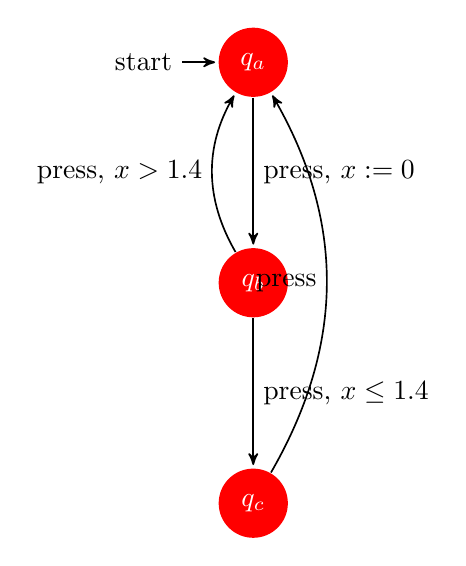
\begin{tikzpicture}[->,>=stealth',shorten >=1pt,auto,node
    distance=2.8cm,
    semithick]
  \tikzstyle{every state}=[fill=red,draw=none,text=white]

  \node[initial,state] (A)                    {$q_a$};
  \node[state]         (B) [below of=A] {$q_b$};
  \node[state]         (C) [below of=B] {$q_c$};
  
  \path (A) edge              node {press, $x:=0$}    (B)
  (B) edge [bend left] node {press, $x > 1.4$}        (A)
  edge              node {press, $x \le 1.4$}         (C)
  (C) edge [bend right] node {press}                  (A);
\end{tikzpicture}

Timed automaton representing a light bulb with two
brightness settings, example taken from \cite{aceto2007reactive}

\begin{itemize}
\item Formally, a timed automaton over a finite set of clocks $C$
  and a finite set of actions $Act$ is a 4-tuple $(L, l_{0}, E, I)$.
\item $L$ is a finite set of locations.
\item $l_{0}$ is the initial location.
\item $E \subseteq L \times B(C) \times Act \times 2^{C} \times L$
  is a finite set of edges.
\item $I: L \rightarrow B(C)$ assigns invariants to each edge
  location.
\item $B(C)$ is the set of clock constraints over C. An element of $B(C)$
  can be an equality, a slack inequality, or a strict inequality on
  $v(x)$ for some $x$ $\epsilon$ $C$, or
  an AND combination of such constraints.
\item The state of the automaton at any particular instant is given
  by the ordered pair $(l, v)$ which gives the location and assigns
  a value to each clock. 
\item A transition is either a delay transition where the automaton
  stays at the same location while advancing each clock by the same
  time delay, or an action transition where the automaton performs a
  state change while resetting some of its clocks.
\end{itemize}

\pagebreak

\section{Timed relations on timed automata}

\subsection{Time abstracted bisimilarity}

\begin{itemize}
  
\item \emph{Strong time abstracted bisimulation}: A binary relation
  $R$ is a strong time abstracted bisimulation (STaB) if and only if, for all
  $(s_1, s_2)$ $\epsilon$ $R$ , $a$ $\epsilon$ $Act $, $d$ $\epsilon$ $R_{\ge 0}$\\
  $\forall s_1' (s_1 \xrightarrow{a} s_1' \Rightarrow \exists s_2'
  . (s_2 \xrightarrow{a} s_2' \wedge (s_1', s_2')$ $\epsilon$ $R ) )
  \wedge $ \\
  $\forall s_2' (s_2 \xrightarrow{a} s_2' \Rightarrow \exists s_1'
  . (s_1 \xrightarrow{a} s_1' \wedge (s_1', s_2')$ $\epsilon$ $R ) ) \wedge $ \\
  $\forall s_1' (s_1 \xrightarrow{d} s_1' \Rightarrow \exists (s_2',
  d')
  . (s_2 \xrightarrow{d'} s_2' \wedge (s_1', s_2')$ $\epsilon$ $R ) )
  \wedge $ \\
  $\forall s_2' (s_2 \xrightarrow{d} s_2' \Rightarrow \exists (s_1', d')
  . (s_1 \xrightarrow{d'} s_1' \wedge (s_1', s_2')$ $\epsilon$ $R ) ) $ \\

\item It can be shown that the union of all strong time abstracted
  bisimulations over the set of (location, valuation) pairs is a
  strong time abstracted bisimulation. This binary relation is called
  \textit{strong time abstracted bisimilarity}.

\item \emph{Time abstracted delay bisimulation}: A binary relation
  $R$ is a time abstracted delay bisimulation (TadB) if and only if, for all
  $(s_1, s_2)$ $\epsilon$ $R$ , $a$ $\epsilon$ $Act $, $d$ $\epsilon$ $R_{\ge 0}$\\
  $\forall s_1' (s_1 \xrightarrow{a} s_1' \Rightarrow \exists (s_2', d)
  . (s_2 \xrightarrow{d} \xrightarrow{a} s_2' \wedge (s_1', s_2')$ $\epsilon$ $R ) )
  \wedge $ \\
  $\forall s_2' (s_2 \xrightarrow{a} s_2' \Rightarrow \exists (s_1', d)
  . (s_1 \xrightarrow{d} \xrightarrow{a} s_1' \wedge (s_1', s_2')$
  $\epsilon$ $R ) ) 
  \wedge $ \\
  $\forall s_1' (s_1 \xrightarrow{d} s_1' \Rightarrow \exists (s_2',
  d')
  . (s_2 \xrightarrow{d'} s_2' \wedge (s_1', s_2')$ $\epsilon$ $R ) )
  \wedge $ \\
  $\forall s_2' (s_2 \xrightarrow{d} s_2' \Rightarrow \exists (s_1', d')
  . (s_1 \xrightarrow{d'} s_1' \wedge (s_1', s_2')$ $\epsilon$ $R ) ) $ \\

\item It can be shown that the union of all time abstracted delay
  bisimulations over the set of (location, valuation) pairs is a
  time abstracted delay bisimulation. This binary relation is called
  \textit{time abstracted delay bisimilarity}.

\item \emph{Time abstracted observational bisimulation}: A binary relation
  $R$ is a time abstracted observational bisimulation (TaoB) if and only if, for all
  $(s_1, s_2)$ $\epsilon$ $R$ , $a$ $\epsilon$ $Act $, $d$ $\epsilon$ $R_{\ge 0}$\\
  $\forall s_1' (s_1 \xrightarrow{a} s_1' \Rightarrow \exists (s_2',
  d, d') . (s_2 \xrightarrow{d} \xrightarrow{a} \xrightarrow{d'} s_2'
  \wedge (s_1', s_2')$ $\epsilon$ $R ) ) \wedge $ \\
  $\forall s_2' (s_2 \xrightarrow{a} s_2' \Rightarrow \exists (s_1',
  d, d') . (s_1 \xrightarrow{d} \xrightarrow{a} \xrightarrow{d'} s_1'
  \wedge (s_1', s_2')$ $\epsilon$ $R ) ) \wedge $ \\
  $\forall s_1' (s_1 \xrightarrow{d} s_1' \Rightarrow \exists (s_2',
  d')
  . (s_2 \xrightarrow{d'} s_2' \wedge (s_1', s_2')$ $\epsilon$ $R ) )
  \wedge $ \\
  $\forall s_2' (s_2 \xrightarrow{d} s_2' \Rightarrow \exists (s_1', d')
  . (s_1 \xrightarrow{d'} s_1' \wedge (s_1', s_2')$ $\epsilon$ $R ) ) $ \\

\item It can be shown that the union of all time abstracted observational
  bisimulations over the set of (location, valuation) pairs is a
  time abstracted observational bisimulation. This binary relation is called
  \textit{time abstracted observational bisimilarity}.

\end{itemize}

\section{Abstractions}



\section{Algorithms}

\subsection{Creation of the zone valuation graph}

This algorithm is adapted from the algorithm in
\cite{DBLP:conf/cav/GuhaNA12}. We changed it to make the correctness
more evident. 
In summary, the algorithm consists of a \emph{forward
  propagation} which ensures that all \emph{reachable} zones are created, and a
\emph{backward propagation} which ensures that each zone is \emph{stable} with
respect to its successors. For the forward propagation, we use a queue,
akin to the queue of the classic \emph{breadth-first search} algorithm
for graphs, to traverse the timed automaton, starting from the inital
location, to ensure that all reachable zones are created. In each
queue element (with the exception of the first element containing the
inital location, which has no predecessor), we store a location
$l_{succ}$, its predecessor in the current path $l_{pred}$, and the
transition $t$ from $l_{pred}$ to $l_{succ}$. It should be noted
that this may result in some locations being visited multiple times,
and in unreachable locations never being visited. Each time a location
is visited, we create therein, new zones which are reachable from the
zones of the predecessor. \\
Thus, for each predecessor zone $(l_{pred}, \zeta _{pred_{i}})$, the
derived successor zone is $(l_{succ}, \zeta _{succ_{i}})$, where

\begin{displaymath} 
\zeta _{succ_{i}} = ((\zeta _{pred_{i}} \uparrow \cap t.guard)[t.resets := 0]) \uparrow
\end{displaymath} 

Thus, if we let  $(l_{pred}, \zeta _{pred_{i}})$ range over the
existing zones of $l_{pred}$, and if we let  $(l_{succ}, \zeta
_{succ_{j}})$ range over the existing zones of $l_{succ}$, then the
new zones in $l_{succ}$ will cover

\begin{displaymath} 
\zeta _{succ_{new}} = (\bigcup _{i} \zeta_{succ_{i}}) - (\bigcup _{j} \zeta_{succ_{j}})
\end{displaymath} 

Since $\zeta _{succ_{new}}$ is not necessarily convex, we may need to
split it into multiple convex polyhedra before creating the
corresponding zones in the $l_{succ}$. Then, we split the zones of
$l_{succ}$ to ensure stability with respect to
its invariant and outgoing edge constraints. If any new
zones are thus created, we enqueue each of the location's successors,
in order to ensure that all reachable zones are created. The forward
propagation ends when the queue is empty. In the backward propagation, we
iterate through the transitions of the timed automaton, multiple times
if necessary, splitting the zones of the source of each transition
with respect to the zones of the transition's target, until we achieve
stability of each zone of each location. This generates the zone
valuation graph.

\begin{algorithm2e}[H]
  Initialise the queue $Q$ with a single element $(null, null, l_0)$\;
  Initialise the graph $zone\_graph$ with a single node $(l_0, v_0 \uparrow)$
  with an $\epsilon$ self-loop\;
  \While{$Q$ is not empty}{
    Dequeue $(l_{parent}, transition, l_{child})$ from $Q$\;
    \If{$l_{parent} \neq null$}{
      \ForEach{zone $Z_{parent}$ of $l_{parent}$}{
        Add new zones to the zones of $l_{child}$ so that all zones
        reachable from $Z_{parent}$ (given by the equation $Z_{child}
        = (((Z_{parent} \uparrow ) \cap transition.guard)
        [transition.resets := 0]) \uparrow$) are represented\;
        Abstract if necessary\;
        Update edges from $Z_{parent}$ to the new zones of $l_{child}$
        \If{new zones are created in $l_{child}$}{
          \ForEach{outgoing transition $t$ of $l_{child}$}{
            Enqueue $(l_{child}, t, t.target)$ in $Q$\;
          }
        }
      }
    }
    Set $new\_zone$\;
    \While{$new\_zone$}{
      Reset $new\_zone$\;
      \ForEach{transition $t$ in the timed automaton}{
        Split the zones of $t.source$ to be stable with respect to the
        zones of $t.target$, so that each source zone $Z_{parent}$
        with an edge to a target zone $Z_child$ satisfies $Z_{parent}
        \subseteq t.guard \cap ([t.resets := 0]Z_{child})$\;
        Update edges accordingly\;
        \If{new zones are created in $t.source$}{
          Set $new\_zone$\;
        }
      }
    }
  }
  Return $zone\_graph$\;
\end{algorithm2e}

\begin{itemize}

\item \texttt{Termination}: The algorithm, in the worst case,
  will create as many zones as there are regions in the region graph,
  as the region graph abstraction ensures that the number of zones
  cannot exceed the number of regions. Since the number of regions is
  known to be bounded, termination of the algorithm is
  guaranteed.

\item \texttt{Reachability}: Since the initial zone is the future of
  the zero valuation in the initial zone, it is reachable by
  definition. A new zone is only created when it is reachable from some
  zone which has already been created, thus each zone which is created
  is reachable by induction.

\item \texttt{Stability}: Since the termination of the backward
  propagation step only occurs after an iteration in which all the
  edges of the timed automaton are traversed without causing any
  splitting of states, it follows that the zone graph is stable with
  respect to itself after this last iteration.

\end{itemize}

\bibliographystyle{ieeetr}
\bibliography{thesis}

\end{document}
